\documentclass[9pt]{article}

\usepackage[utf8]{inputenc}
\usepackage{geometry}
\geometry{
    a4paper,
    total={170mm,257mm},
    left=15mm,
    right=15mm,
    top=20mm,
    bottom=20mm,
}
\usepackage{multicol}
\usepackage[font=small,labelfont=bf]{caption}
\setlength{\columnsep}{0.25cm}
\usepackage[inline]{enumitem}
\usepackage{amssymb}
\usepackage{xcolor}
\usepackage{mathtools} 
\setlength{\parindent}{0em}
\setlength{\parsep}{0em}
\usepackage{tikz}
\setlength{\parskip}{0em}
\usetikzlibrary{decorations.pathmorphing,patterns}
\usepackage[american,cuteinductors]{circuitikz}
\usetikzlibrary{shapes,arrows,circuits,calc,babel}
% Definition of blocks:
\tikzset{%
  block/.style    = {draw, thick, rectangle, minimum height = 3em,
    minimum width = 3em},
  sum/.style      = {draw, circle, node distance = 2cm}, % Adder
  input/.style    = {coordinate}, % Input
  output/.style   = {coordinate} % Output
}
% Defining string as labels of certain blocks.
\newcommand{\suma}{\Large$+$}
\newcommand{\inte}{$\displaystyle \int$}
\newcommand{\derv}{\huge$\frac{d}{dt}$}

\def\mf{\ensuremath\mathbf}
\def\mb{\ensuremath\mathbb}
\def\mc{\ensuremath\mathcal}
\def\lp{\ensuremath\left(}
\def\rp{\ensuremath\right)}
\def\lv{\ensuremath\left\lvert}
\def\rv{\ensuremath\right\rvert}
\def\lV{\ensuremath\left\lVert}
\def\rV{\ensuremath\right\rVert}
\def\lc{\ensuremath\left\{}
\def\rc{\ensuremath\right\}}
\def\ls{\ensuremath\left[}
\def\rs{\ensuremath\right]}
\def\bmx{\ensuremath\begin{bmatrix*}[r]}
\def\emx{\ensuremath\end{bmatrix*}}
\def\bmxc{\ensuremath\begin{bmatrix*}[c]}
\def\emxc{\ensuremath\end{bmatrix*}}
% \def\t{\lp t\rp}
% \def\k{\ls k\rs}

\newcommand{\demoex}[2]{\onslide<#1->\begin{color}{black!60} #2 \end{color}}
\newcommand{\demoexc}[3]{\onslide<#1->\begin{color}{#2} #3 \end{color}}
\newcommand{\anim}[3]{\onslide<#1->{\begin{color}{#2!60} #3 \end{color}}}
\newcommand{\ct}[1]{\lp #1\rp}
\newcommand{\dt}[1]{\ls #1\rs}

\renewcommand{\familydefault}{\sfdefault}

\begin{document}
\begin{center}
\begin{Large}
\textbf{Linear Systems: LDS Solution, Stability, Controllability \&  Observability Assignment}
\end{Large}
\end{center}
\vspace{0.2cm}

\begin{multicols}{2}

\begin{enumerate}[resume]
    \item Consider $\mf{A} = \bmx 1 & 1 & 0\\ 0 & 0 & 1\\ 0 & 0 & 1\emx$. Compute $\mf{A}^{100}$ and $e^{t\mf{A}}$.

    \item Assuming that $\mf{A} \in \mb{R}^{n \times n}$ is diagonalizable with eigenvalues $\lambda_1, \lambda_2,\ldots \lambda_n$. Prove that the eigenvalues of $e^{\mf{A}}$ are $e^{\lambda_1}, e^{\lambda_2}, \ldots e^{\lambda_n}$

    \item Consider a linear time-variant discrete-time, $\mf{x}\dt{k+1} = \mf{A}\dt{k}\mf{x}\dt{k} + \mf{B}\dt{k}\mf{u}\dt{k}$. Find the general expression for the zero-input solution, and the zero-state solution.

    \item What are the conditions on the individual LTI discrete-time systems $H_1\ct{z}$ and $H_2\ct{z}$ for the following overall system to be:
    \begin{enumerate*}
        \item internally stable;
        \item externally stable;
        \item controllable; and
        \item observable
    \end{enumerate*}
    \begin{center}
        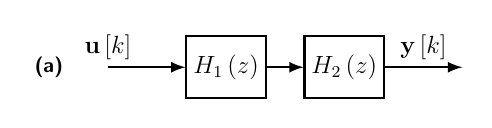
\begin{tikzpicture}[scale=0.75, transform shape, thick, node distance=2cm]
        \draw
            node [input, name=input1] {} 
            node [block, right of=input1] (sys1) {{\large $H_1\ct{z}$}}
            node [block, right of=sys1] (sys2) {{\large $H_2\ct{z}$}}
            node [input, right of=sys2, name=output1] {};
            \draw[-latex] node [above] {{\large $\mf{u}\dt{k}$}} (input1) -- node {} (sys1);
            \draw[-latex](sys1) -- node {} (sys2);
            \draw[-latex](sys2) -- node[above] {\large $\mf{y}\dt{k}$} (output1);
            \node[]  at (-1,0) {\textbf{(a)}};
        \end{tikzpicture}

        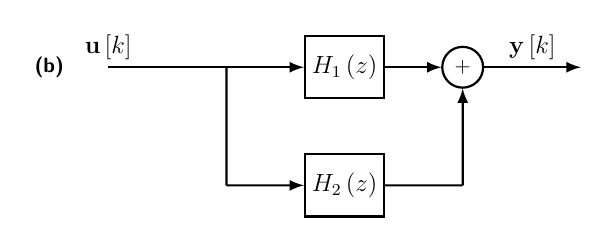
\begin{tikzpicture}[scale=0.75, transform shape, thick, node distance=2cm]
        \draw
            node [input, name=input1] {}
            node [input, right of=input1, name=tempin1] {} 
            node [input, below of=tempin1, name=tempin2] {} 
            node [block, right of=tempin1] (sys1) {{\large $H_1\ct{z}$}}
            node [block, right of=tempin2] (sys2) {{\large $H_2\ct{z}$}}
            node [sum, right of=sys1] (suma1) {$\suma$} 
            node [input, right of=sys2, name=tempout2] {}
            node [input, right of=suma1, name=output1] {};

            \draw[-] node [above] {{\large $\mf{u}\dt{k}$}} (input1) -- node {} (tempin1);
            \draw[-latex] node {} (tempin1) -- node {} (sys1);
            \draw[-] node {} (tempin1) -- node {} (tempin2);
            \draw[-latex] node {} (tempin2) -- node {} (sys2);
            \draw[-latex](sys1) -- (suma1);
            \draw[-] node {} (sys2) -- node {} (tempout2);
            \draw[-latex] node {} (tempout2) -- node {} (suma1);
            \draw[-latex] node {} (suma1) -- node[above] {\large $\mf{y}\dt{k}$} (output1);
            \node[]  at (-1,0) {\textbf{(b)}};
        \end{tikzpicture}

        % \begin{tikzpicture}[scale=0.75, transform shape, thick, node distance=2cm]
        % \draw
        %     node [input, name=input1] {}
        %     node [sum, right of=input1] (suma1) {$\suma$} 
        %     node [input, below of=suma1, name=tempfb] {} 
        %     node [block, right of=suma1] (sys1) {{\large $H_1$}}
        %     node [input, right of=sys1, name=tempout1] {}
        %     node [input, right of=tempout1, name=output1] {}
        %     node [input, below of=tempout1, name=tempout2] {}
        %     node [block, below of=sys1] (sys2) {{\large $H_2$}};

        %     \draw[-latex] node [above] {{\large $\mf{u}\ct{t}$}} (input1) -- node {} (suma1);
        %     \draw[-latex] node {} (suma1) -- node {} (sys1);
        %     \draw[-] node {} (sys1) -- node {} (tempout1);
        %     \draw[-latex] node {} (tempout1) -- node {} (output1);
        %     \draw[-] node {} (tempout1) -- node {} (tempout2);
        %     \draw[-latex] node {} (tempout2) -- node {} (sys2);
        %     \draw[-] node {} (sys2) -- node {} (tempin2);
        %     \draw[-latex] node {} (tempin2) -- node {} (suma1);
        %     \draw[-latex] node {} (tempout1) -- node[above] {\large $\mf{y}\ct{t}$} (output1);
        %     \node[]  at (-1,0) {\textbf{(c)}};
        % \end{tikzpicture}
    \end{center}

    \item Consider a the LTI system, $\dot{\mf{x}}\ct{t} = \mf{A}\mf{x}\ct{t}$, where $\mf{A} \in \mb{R}^{n \times n}$. An experiment was carried out with this system, where the system was started at different initial conditions $\mf{x}_i\ct{0^-}$, and the corresponding state trajectories were recorded to be $\mf{x}_i\ct{t}, \,\, \forall t \geq 0$. Assuming that the set of initial conditions$\lc \mf{x}\ct{0^-} \rc_{i=1}^n$ are linearly independent, find the expression for the $e^{t\mf{A}}$.

    \item Consider the following system, where the input is the force $f$ applied to mass $m_2$, and the output of the system, positions of masses $m_1$ and $m_2$, are measured using a set of position sensors. Assume $m_1 = m_2 = 1Kg$, $k_1 = k_2 = 1 Nm^{-1}$, and $b_1 = b_2 = 1 Nm^{-1}s$.
    \begin{enumerate}
        \item Is this system controllable? Is the system still controllable if the input $f$ was acting on the mass $m_1$ instead of $m_2$?
        \item Is this system observable? If instead of measuring both position $x_1$ and $x_2$, if the output of the system was either $x_1$ or $x_2$, is the system still observable?
    \end{enumerate}
    \begin{center}
    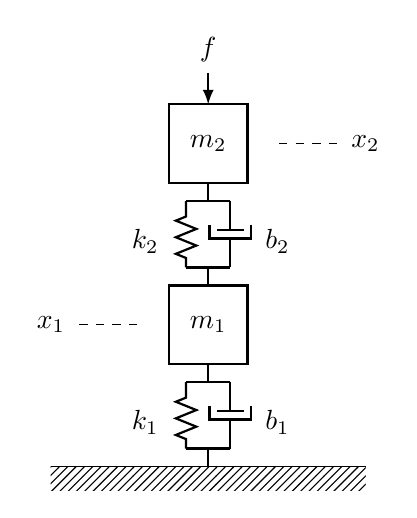
\begin{tikzpicture}[every node/.style={draw,outer sep=0pt,thick}, scale=0.8]
    %define the spring
    \tikzstyle{spring}=[thick,decorate,decoration={zigzag,pre length=0.12cm,post length=0.12cm,amplitude=1.3mm,segment length=6}]

    %define the dashpot
    \tikzstyle{damper}=[thick,decoration={markings,
      mark connection node=dmp,
      mark=at position 0.5 with 
      {
          \node (dmp) [thick,inner sep=0pt,transform shape,rotate=-90,minimum width=15pt,minimum height=3pt,draw=none] {};    
          \draw [thick] ($(dmp.north east)+(2pt,0)$) -- (dmp.south east) -- (dmp.south west) -- ($(dmp.north west)+(2pt,0)$);
          \draw [thick] ($(dmp.north)+(0,-5pt)$) -- ($(dmp.north)+(0,5pt)$);
      }
    }, decorate]

    %define the spring-dashpot
    \tikzstyle{spr-dash}=[thick,decorate,decoration={markings,
      mark connection node=sqr,
      mark=at position 0.5 with
      {
          \node (sqr) [thick,minimum width=16pt,minimum height=24pt,draw=none] {};
          \draw [thick] (sqr.north west) -- (sqr.north east);
          \draw [thick] (sqr.south west) -- (sqr.south east);
          \draw [spring] (sqr.south west) -- (sqr.north west);
          \draw [damper] (sqr.south east) -- (sqr.north east);
      }
      }]

    %define the ground
    \tikzstyle{ground}=[fill,pattern=north east lines,draw=none,minimum width=0.75cm,minimum height=0.3cm]

    \begin{scope}[xshift=5.5cm]
    %draw the frame mass
    \node (M1) [minimum width=1cm,minimum height=1cm] {$m_1$};
     
    %draw the vehicle mass
    \node (M2) at (M1.north) [yshift=+1.8cm, minimum width=1cm, minimum height=1cm] {$m_2$};

    \node (ground-medium) at (M1.south) [ground,yshift=-1.3cm,minimum width=4cm,anchor=north] {};
    \draw (ground-medium.north west) -- (ground-medium.north east);

    \draw [spr-dash] (ground-medium.north) -- (M1.south);
    \node [draw=none] at ($(ground-medium.north)+(-1cm,0.7cm)$) {$k_{1}$};
    \node [draw=none] at ($(ground-medium.north)+(1.1cm,0.7cm)$) {$b_{1}$};
    \draw [spr-dash] (M1.north) -- (M2.south);
    \node [draw=none] at ($(M1.north)+(-1.0cm,0.7cm)$) {$k_{2}$};
    \node [draw=none] at ($(M1.north)+(1.1cm,0.7cm)$) {$b_{2}$};
     
    \draw [-latex,thick] (M2.north) ++ (0, 0.5cm) -- (M2.north);
    \draw [dashed,thin] (M2.east) ++ (0.5cm, 0) -- +(1.0cm, 0);
    \node [draw=none, right] at ($(M2.east) + (1.5cm, 0)$) {$x_{2}$};

    \draw [dashed,thin] (M1.west) ++ (-0.5cm, 0) -- +(-1.0cm, 0);
    \node [draw=none, left] at ($(M1.west) + (-1.5cm, 0cm)$) {$x_{1}$};

    \node [draw=none, yshift=0.7cm] at (M2.north) {$f$};
    \end{scope}
    \end{tikzpicture}
    \end{center}

    Assume now that instead of $f$ acting on $m_2$, it was acting on $m_1$, and the output of interest was the acceleration of the mass $m_1$. What would be correspondoing state and measurement equations in this case? Is this system still controllable and observable?

    \item Write down the state and measurement equations of the following system, assuming the the output being measured are the positions of the masses $m_1$ and $m_2$. Assuming that $\frac{k_1}{m_1} = \frac{k_2}{m_2}$, is the system controllable? If $\frac{k_1}{m_1} \neq \frac{k_2}{m_2}$, is the system now controllable? Why are these two systems different in terms of controllability?

    \begin{center}
    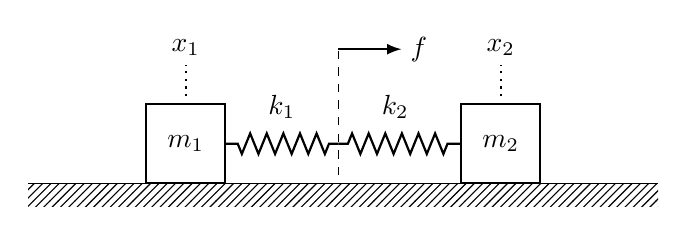
\begin{tikzpicture}[every node/.style={draw,outer sep=0pt,thick}, scale=0.8]
    %define the spring
    \tikzstyle{spring}=[thick,decorate,decoration={zigzag,pre length=0.12cm,post length=0.12cm,amplitude=1.3mm,segment length=6}]

    %define the dashpot
    \tikzstyle{damper}=[thick,decoration={markings,
      mark connection node=dmp,
      mark=at position 0.5 with 
      {
          \node (dmp) [thick,inner sep=0pt,transform shape,rotate=-90,minimum width=15pt,minimum height=3pt,draw=none] {};    
          \draw [thick] ($(dmp.north east)+(2pt,0)$) -- (dmp.south east) -- (dmp.south west) -- ($(dmp.north west)+(2pt,0)$);
          \draw [thick] ($(dmp.north)+(0,-5pt)$) -- ($(dmp.north)+(0,5pt)$);
      }
    }, decorate]

    %define the spring-dashpot
    \tikzstyle{spr-dash}=[thick,decorate,decoration={markings,
      mark connection node=sqr,
      mark=at position 0.5 with
      {
          \node (sqr) [thick,minimum width=16pt,minimum height=24pt,draw=none] {};
          \draw [thick] (sqr.north west) -- (sqr.north east);
          \draw [thick] (sqr.south west) -- (sqr.south east);
          \draw [spring] (sqr.south west) -- (sqr.north west);
          \draw [damper] (sqr.south east) -- (sqr.north east);
      }
      }]

    %define the ground
    \tikzstyle{ground}=[fill,pattern=north east lines,draw=none,minimum width=0.75cm,minimum height=0.3cm]

    \begin{scope}[xshift=5.5cm]
    %draw the frame mass
    \node (M1) [minimum width=1cm,minimum height=1cm] {$m_1$};
     
    %draw the vehicle mass
    \node (M2) at (M1.east) [xshift=+3.5cm, minimum width=1cm, minimum height=1cm] {$m_2$};

    \node (ground-medium) at (M1.south) [ground,yshift=0cm,minimum width=4cm,anchor=north] {};
    \draw (ground-medium.north west) -- (ground-medium.north east);

    \node (ground-medium) at (M2.south) [ground,yshift=0cm,minimum width=4cm,anchor=north] {};

    \draw (ground-medium.north west) -- (ground-medium.north east);

    \draw [spring] (M1.east) ++ (1.8cm,0.0cm) -- (M1.east);
    \draw [spring] (M1.east) ++ (1.8cm,0.0cm) -- (M2.west);
    
    \draw [dashed,thin] (M1.east) ++ (1.8cm,-0.5cm) --  +(0cm,2cm);
    \draw [thick,-latex] (M1.east) ++ (1.8cm,1.5cm) --  +(1cm,0cm);
    \node [draw=none, right] at ($(M1.east) + (2.8cm,1.5cm)$) {$f$};
    \node [draw=none, above] at ($(M1.east) + (0.9cm,0.25cm)$) {$k_1$};
    \node [draw=none, above] at ($(M1.east) + (2.7cm,0.25cm)$) {$k_2$};
    \draw [dotted,thick] (0, 0.75) --  +(0cm,0.5cm);
    \node [draw=none, above] at (0, 1.25) {$x_1$};
    \draw [dotted,thick] (5.0cm, 0.75) --  +(0cm,0.5cm);
    \node [draw=none, above] at (5.0, 1.25) {$x_2$};
    \end{scope}
    \end{tikzpicture}
    \end{center}

    \item Consider the following system,
    \[ \begin{split}
        \mf{x}[n + 1] &= \bmx a & b \\ c & d\emx \mf{x}[n] + \bmx 1 \\ 1\emx \mf{u}[n] \\
        \mf{y}[n] &= \bmx 1 & 0\emx \mf{x}[n]
       \end{split} \]
    Determine the conditions $a, b, c, $ and $d$ for complete state controllability and complete observability.

    \item Consider the following system,
    \[ \mf{x}[n + 1] = \bmx 0 & 1 \\ -0.16 & 1\emx \mf{x}[n] + \bmx 1 \\ 0.5\emx \mf{u}[n] \]
    \[ \mf{x}[0] = \bmx 1 \\ -1\emx \]
    Verify that this system is controllable. Determine the sequence of input signal $\mf{u}[0]$ and $\mf{u}[1]$ such that $\mf{x}[2] = \bmx -1 \\ 2 \emx$.

    \item Consider the following system,
    \[ \begin{split}
        \mf{x}[n + 1] &= \bmx 0 & 1 \\ -0.16 & 1\emx \mf{x}[n] + \bmx 0 \\ 1\emx \mf{u}[n] \\
        \mf{y}[n] &= \bmx 1 & 1\emx \mf{x}[n]
        \end{split} \]
    Verify that this system is observable.
    \newpage
\end{enumerate}

\end{multicols}
\end{document}